
%(BEGIN_QUESTION)

\large \textbf{Praktisk øving på brødbrett - Oppkobling av sinking og sourcing PLS inngang}
\normalsize 
\vskip 10pt 
I denne øvingen skal du bruke et koblingsbrett for å koble en motstand i serie med en lysdiode. Verdien til motstanden skal du beregne i oppgaven. 

\vskip 10pt 
\large \textbf{Utstyr du trenger}

\vskip 10pt 
\begin{itemize}[noitemsep]

\item 24V industristrømforsyning
\item Koblingsbrett
\item Isolert ledning
\item Motstand med ukjent verdi 
\item Lysdiode
\item Amperemeter
\item Voltmeter
\item Ohmmeter
\end{itemize}


\large \textbf{Kretsen}
\normalsize
\vskip 10pt 
$$\includegraphics[width=10cm]{i04881.eps}$$
Lysdioden du har fått utdelt skal skal trekke en strøm på 7mA og vil da ha en spenning på ca. 1.7 V over seg. 
Oppgaver:
\begin{itemize}[noitemsep]
	\item Regn ut hvilken verdi seriemotstanden må ha. 
	\item Motstandere kommer med verdier i faste intervaller, velg ut den nærmeste og koble denne i serie med lysdioden. (NB. strømmen i en diode går fra anoden til katoden. Anoden er det lengste benet. )
	\item Koble et amperemeter inni kretsen og mål strømmen. Stemmer det med den beregnede strømmen. 
\end{itemize}


\underbar{file i04880}
%(END_QUESTION)





%(BEGIN_ANSWER)


%(END_ANSWER)





%(BEGIN_NOTES)



%INDEX% Electronics review: series-parallel circuits

%(END_NOTES)


